\section{Bitcoin}
%citations to Mastering Bitcoin, bitcoinwiki, Szabo and Nakamoto
%Transaction flow, mining, cryptoeconomics, network stability, overhead, slow, secure.
% Cryptoeconomics, incentive compatibility through mining fees and BTC minting.
\subsection{Overview}
Bitcoin is a payment network protocol that enables \acrshort{p2p} payments in a sense that no central authority issues new money or tracks transactions. A record of all transactions is held in a shared ledger, where each transaction is verifiable, transparent and can be tracked through all its history. Batches of transactions with a timestamp are called blocks and each block is cryptographically connected to its previous block by including the hash of the previous block. In that manner, a chronological data structure is created, containing verifiable transactions, or else money, that can be spent by the owner's keys. 

Bitcoin's blockchain is secured through repeated computations or else sealed with energy expenditure. The end product is a network that does not need any intermediaries, transactions are made in a \acrshort{p2p} fashion and the blockchain through all this energy expenditure becomes secure and immutable.   


Lets assume that Alice wants to send \bitcoin 7 (bitcoins) to Bob. Alice has already \bitcoin10, she creates a transaction with one input and 2 outputs, one for Bob at \bitcoin7 and one to her address for the change at \bitcoin 2.995 and the rest \bitcoin 0.005 are fees to the miners (today's fees are \bitcoin 0.00005000)\cite{btcfees} to get her transaction into a block. The output for Bob is signed with his public key and the output to her address as change is signed with her private key. After the creation of the transaction, it propagates through nodes in the network, with a gossip protocol, where each node upon receiving it validates it and gossips it to other connected nodes. Finally, it ends up to a node which will include it in the next block that it will successfully mine \cite{btc-wiki-transaction}.

Every node is capable of putting transactions they choose in a block and mine it, but nowadays mining is done collectively and the mining pool chooses the transactions for the next block from the transaction pool \cite{pool-statistics}. Now that there is a block candidate with ordered transactions in it, it is repeatedly hashed by changing an additional value called the nonce. After many changes, a hash is found that is smaller than the difficulty target. A legit block nowadays needs to start with 18 zeros. 

Difficulty adjusts every 2016 blocks and it targets the whole network to produce 2016 blocks every two weeks \cite{difficulty}. An interesting fact is that intervals between finding the next block follow a probability distribution that is memoryless. Block times follow the exponential distribution and the probability of a block \textbf{not} being found in $x$ minutes or longer is: 
\begin{equation}
\label{eq:p(x)}
    p(x) = e^{-(x/10)}
\end{equation}
So that means that finding a block in 10 minutes or less gives as a probability of 0.63, calculating for $x=10$ in \ref{eq:p(x)}. The number of blocks that are expected to be found in a certain time (e.g 2016 per two weeks) follow a Poisson process. The probability of finding $k$ blocks in $T$ minutes is:
\begin{equation}
    P(k,T) = ({\frac{T}{10}})^k \times \frac{e^-({T/10})}{k!}
\end{equation}
So the probability of finding exactly six blocks in an hour would be 0.16 \cite{bowden2018block}.
%https://www.reddit.com/r/btc/comments/6v5ee7/block_times_and_probabilities/

\subsection{Transactions and UTXO}
In this subsection, we elaborate on transactions and the \acrfull{utxo} set.

Transactions are the most important part of every blockchain network, they are the fuel that change the state of the blockchain. At a high level, a transaction is the authorization of a value from the owner to the recipient. Then, the new owner becomes capable of spending this new value by creating a new transaction and transferring ownership of the value. The most common transaction form for bitcoin is a single payment as seen in a simplified\footnote{The difference in the input and output value is the transaction fee.} manner in \ref{fig:btc-tx}. At a lower level, one input contains the digital signature and public key\footnote{The sender's public key is used to verify the digital signature.}, the output to the recipient is signed with recipient's public key.
\begin{figure}[h]
    \centering
    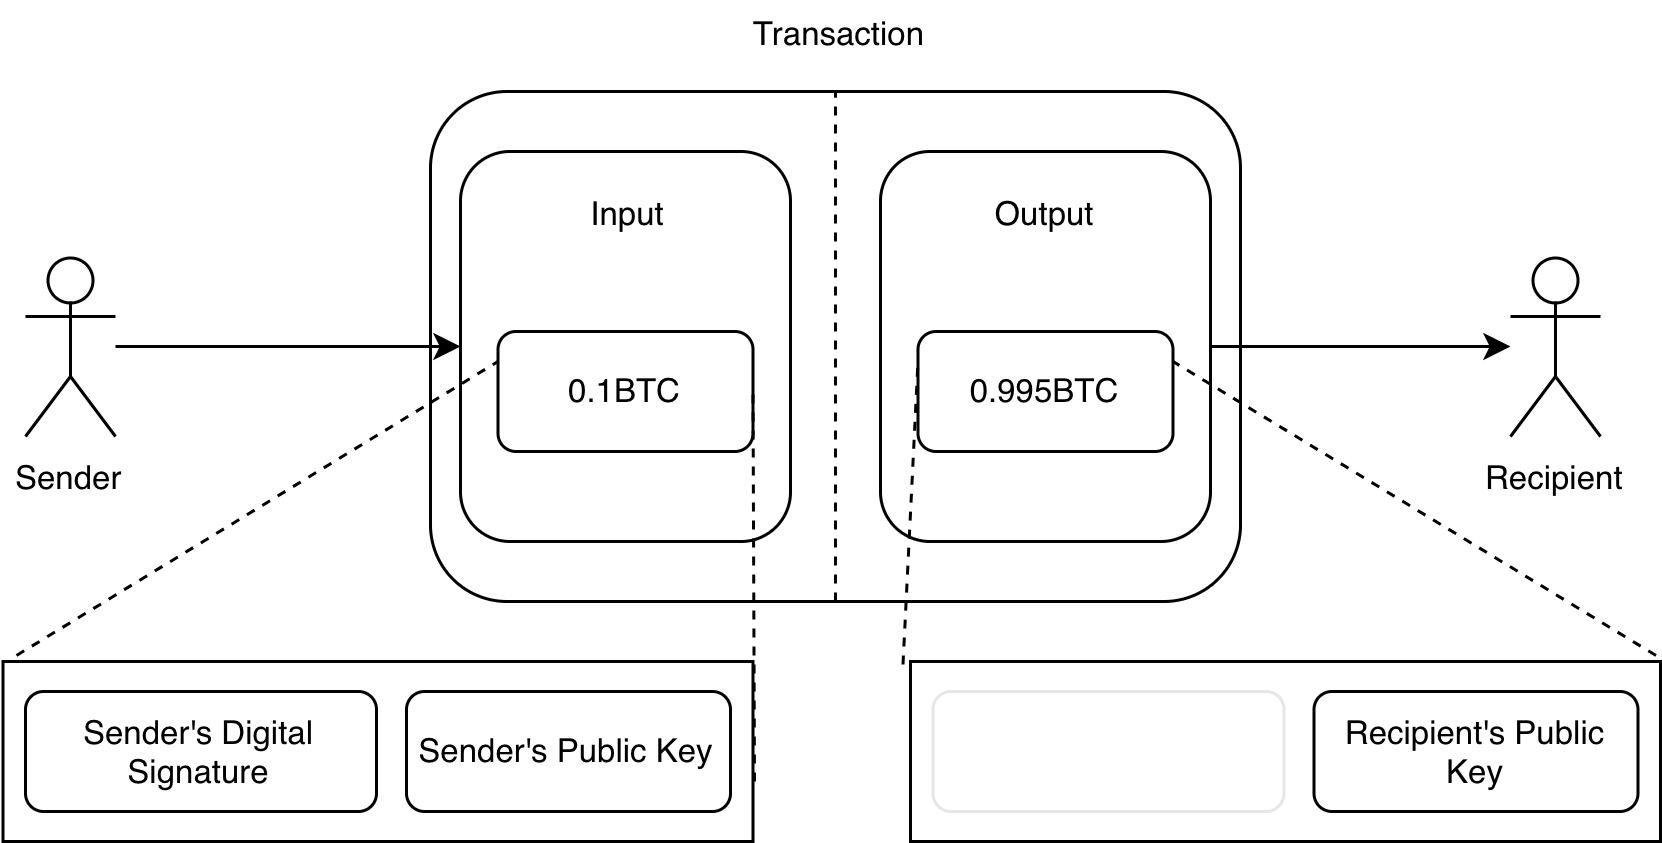
\includegraphics[width=1\textwidth]{images/btc-tx.png}
    \caption{A simplified single transaction with one input and one output.}
    \label{fig:btc-tx}
\end{figure}

The fundamental building block of Bitcoin transactions is the \acrshort{utxo} set. This set, consists of \acrshort{utxo}s that are being used as an input to the next transaction. Each \acrshort{utxo} could be described as an instance of a coin, having any arbitrary value, indivisible, that is going to be spent altogether, destroyed and another new \acrshort{utxo} will take its place. Each \acrshort{utxo} that is consumed as an input to a transaction will create a new one. The relationship of inputs(M) and outputs(N) is $M-N $ where $M,N\geq1$ . Wallets track within the \acrshort{utxo} set, which \acrshort{utxo}s the user's private keys can control, and represents it as a balance. A transaction references previous outputs as new inputs and assigns all inputs to new outputs as seen in \ref{fig:utxo}\footnote{Fees have been excluded for simplicity.}.
\begin{figure}[h]
    \centering
    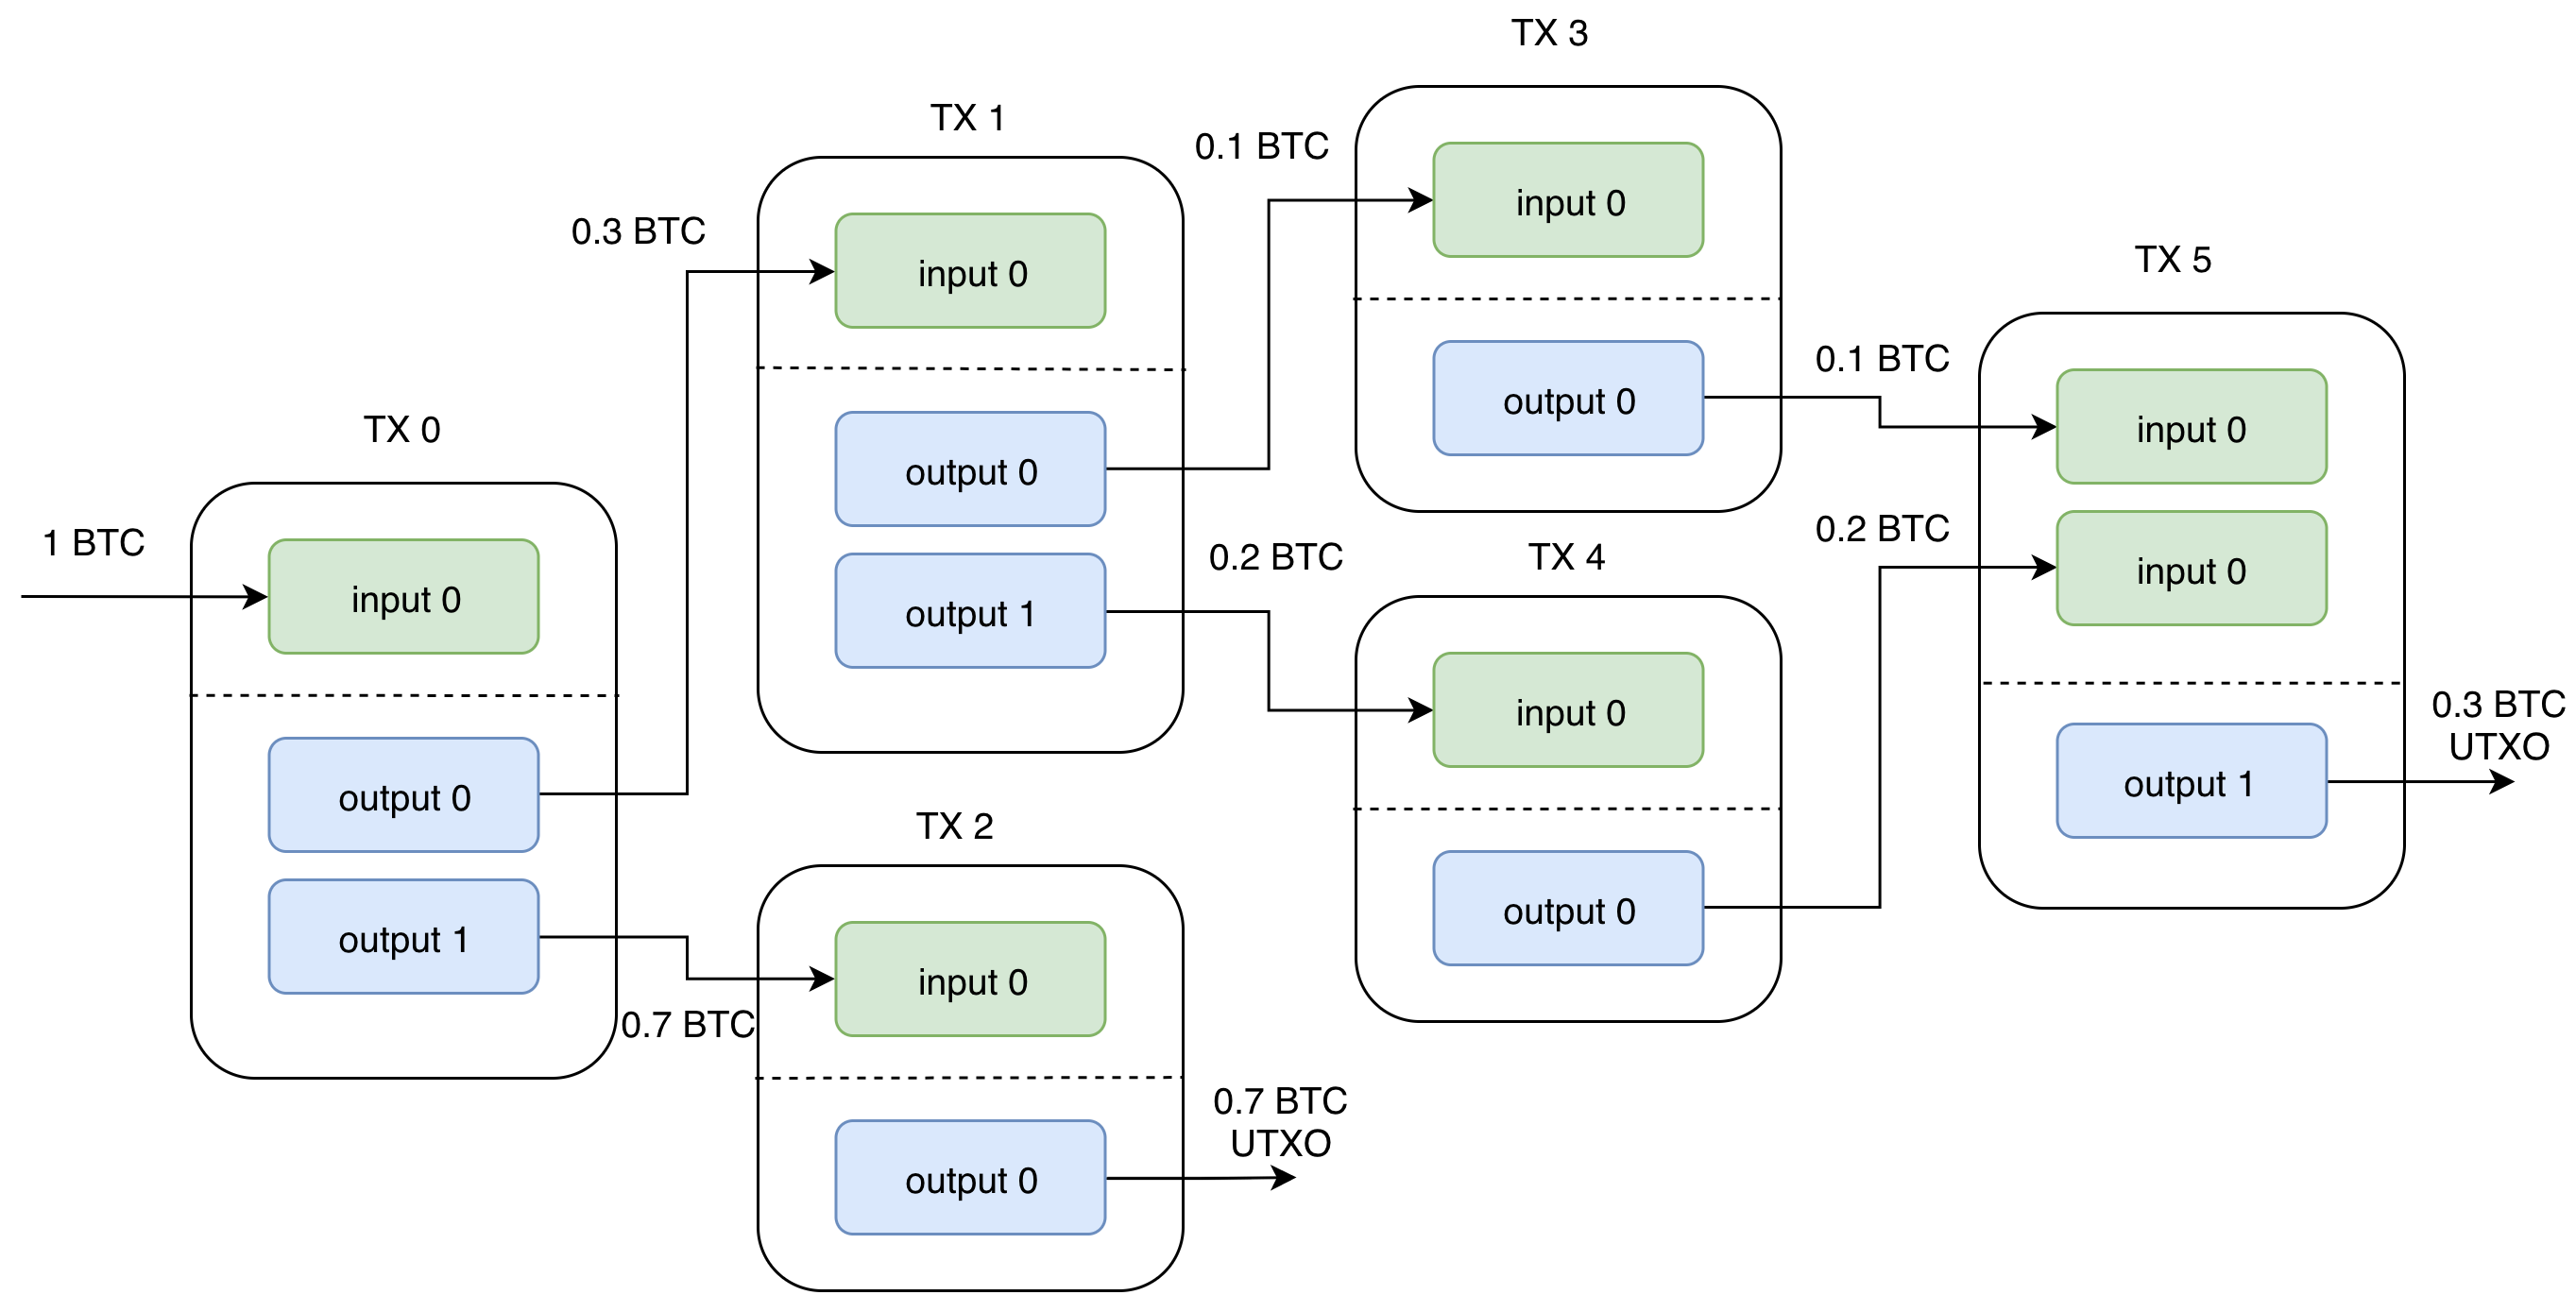
\includegraphics[width=1\textwidth]{images/utxo.png}
    \caption{\acrshort{utxo}s become input to the next transaction.}
    \label{fig:utxo}
\end{figure}

To conclude with \acrshort{utxo}s, we should emphasize their crucial characteristics. Each \acrshort{utxo} is discrete, indivisible, of arbitrary value, denominated in satoshis\footnote{Satoshi is the smallest unit of bitcoin, \bitcoin$10^{-9}$.} The only way to be spent is to be consumed in their entirety by a transaction.
\subsection{The Blockchain}
In this subsection, we elaborate on the abstract idea of blockchain.

An ever-growing distributed list of records, append only, replicated and shared among the participants of the network (aka distributed ledger). Each block in the chain contains a list of transactions and a hash of the previous block. Blockchain is a log whose records are batched into time-stamped blocks where each block is identified by its hash. By including the hash of the previous block\footnote{The Genesis block, is the first block on the chain and it does not include a reference to a previous block.}, it establishes a link between the blocks, thus creating a block-chain. 
	\begin{figure}[H]
	    \centering
	    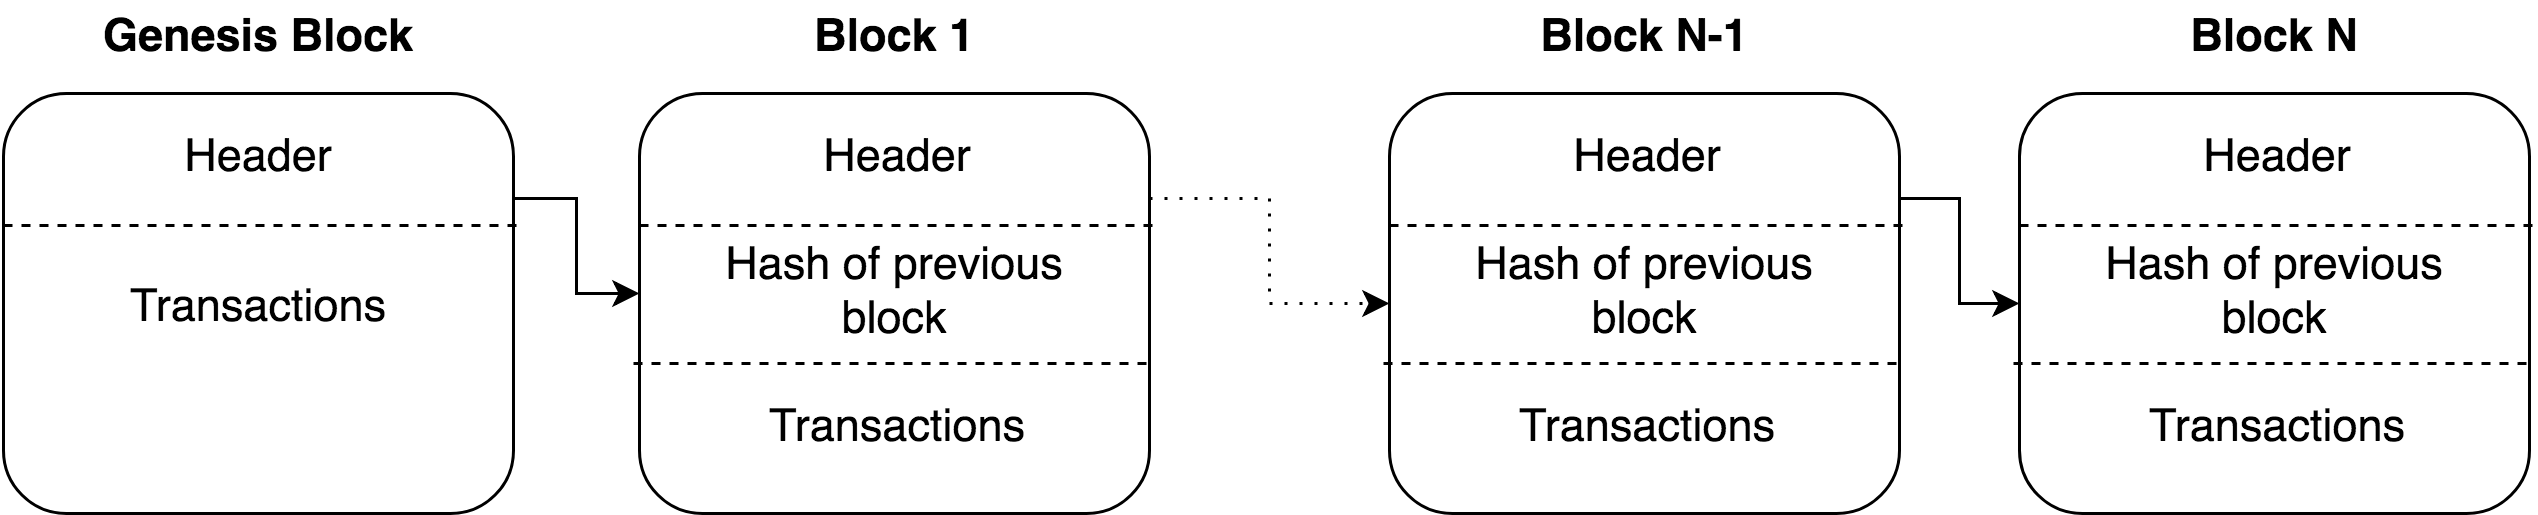
\includegraphics[width=1\textwidth]{images/blockchain_simplified.png}
	    \caption{Blockchain simplified}
	    \label{fig:block_simpl}
	\end{figure}
A blockchain can be defined as an immutable shared ledger that holds transactions, maintained within a decentralized and distributed network of mutually non-trusting peers. Every peer maintains their copy of the ledger and is responsible of validating each transaction on it.

\subsection{Mining and immutability}
In this subsection, we discuss how \acrshort{pow} works and makes the blockchain immutable. We should state that mining, \acrshort{pow} and consensus are highly interrelated. 

Abstractly, every node, receives a transaction, verifies it and propagates it to the rest of the network. This transaction, will eventually be included to a candidate block and finally this block will be part of the blockchain. The bitcoin's system of trust is based on computations through mining which secures the system and enables the emergence of network-wide consensus without central authority. 

Bitcoin uses a consensus algorithm that involves mining and \acrshort{pow}. With \acrshort{pow}, the goal is to find a hash of a block that is lower than the difficulty target; the procedure of hashing the block repeatedly to find a suitable hash is called \textit{mining}. As stated before, mining is done collectively and the hashrate across the entire bitcoin network is 46,000 Peta\footnote{$46000 \times 10^{15}$ hashes per second} hashes per second \cite{btc-hashrate}. The network repeatedly hashes the header of the block, using the SHA256 algorithm. The output of each hash is random and finding a hash below the target is probabilistic. It is similar to rolling a dice that will be under 6, easy, it becomes harder as the goal number becomes lower, e.g numbers only under 2.

With the passing of time, more blocks are added on the blockchain and it becomes infeasible to change its history. If someone wanted to change a block in the past, they would have to recompute the \acrshort{pow} of each next block in order to get matching hashes. 

Finally, the blockchain that is accepted is the longest, heaviest, most expensive or the chain with the most work on it\footnote{Work is defined as the sum of the difficulties.}. To conclude, recomputing a new chain is considered impossible due to the energy expenditure and mining hardware\footnote{Bitcoin is mined with ASICs, the most efficient solution.} that is needed. The deeper in history the alteration the more the computations needed to make it the new acceptable version. 